\documentclass[../ESOF_notes.tex]{subfiles}
 
\begin{document} 

\subsection{Scrum}

\begin{figure}[H]
    \centering
    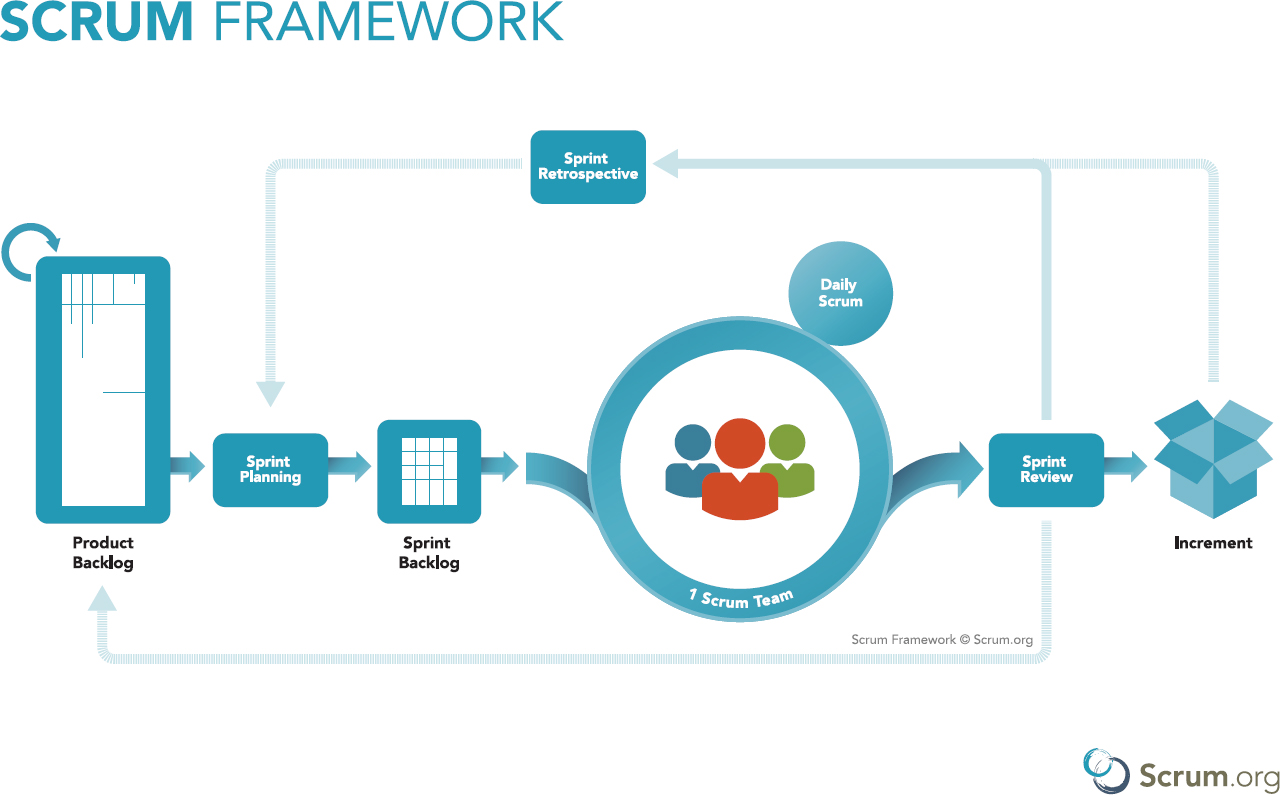
\includegraphics[width=12cm]{ScrumFramework}
    \caption{Scrum Overview}
\end{figure}

\subsubsection{Events}

\begin{itemize}
    \item Sprint planning meeting
    
    Review the features for the next Sprint
    \item Daily scrum
    
    Daily stand-up meeting for coordination and commitment among peers
    \item Sprint review
    
    The team presents what it accomplished during the sprint
    \item Sprint retrospective
    
    Team discusses what they'd like to start/stop/continue doing
\end{itemize}

\subsubsection{Artifacts}

\begin{itemize}
    \item Product backlog
    
    A list of all desired work on the project
    \item Sprint backlog
    
    Shows list of tasks and estimates of work remaining (hours)
    \item Sprint burndown chart
    
    Shows, during a sprint, the total work remaining per day
\end{itemize}

\subsubsection{Roles}

\begin{itemize}
    \item Product Owner
    \begin{itemize}
        \item Define the features of the product and priorities
        \item Decide on release date and content
        \item Accept or reject work results
    \end{itemize}

    \item Scrum Master
    \begin{itemize}
        \item Enact Scrum values and Practices
        \item Remove impediments and external interferences
        \item Ensure that the team is fully functional and productive
    \end{itemize}
    
    \item Development Team
    \begin{itemize}
        \item Does the work
        \item Self-organizing
        \item Typically 5-9 people, ideally full time and multifunctional
    \end{itemize}
\end{itemize}

\subsubsection{Agile Estimation}
\paragraph{User story}
Describes something of value to the user or the system

Example

\textbf{As a} student, \textbf{I want to} indicate preferences for colleagues to share
the same scholar timetable, \textbf{so that} I can be more productive in group works.

\paragraph{Story points}

Relative measure for expressing the “size” of a user story, Influenced by difficulty, risk, complexity, etc.
Typically exponential.

\paragraph{Team velocity}

The number of story points implemented per Sprint

\subsection{eXtreme Programming (XP)}

Developed by Kent Beck.

\subsubsection{Core Values}

\begin{itemize}
    \item Communication
    \item Simplicity
    \item Feedback
    \item Courage
\end{itemize}

\subsubsection{Practices}

\begin{itemize}
    \item The Planning Game
    \begin{enumerate}
        \item The customer comes up with a list of desired features, that are aggregated as user stories (similarly to Scrum).
        \item The developers sort them using story points, so as to know which are easier/harder to implement.
        \item Using this information and project velocity (total story points done per iteration), the customer prioritizes which features to implement.
    \end{enumerate}
    
    \item Small Releases
    
    \begin{itemize}
        \item Start with the smallest useful feature set
        \item Release early and often, adding a few features each time
        \item Releases can be date driven or user story driven
    \end{itemize}
    \item System Metaphor
    
    The system metaphor is a story that everyone - customers, programmers, and managers - can tell
about how the system works.

    \item Simple Design
    
    Use the simplest possible design that gets the job done, so that there are obviously no deficiences
    \item Test-driven Development
    
    Write tests \textit{before} adding a feature, or before fixing a bug. Use unit and acceptance tests.
    \item Refactoring
    
    Improve the structure of the code without changing externally visible behavior (e.g removing duplicate code)

    Refactoring is heavily related to automated tests and simple design.
    \item Pair Programming
    
    Process:
    \begin{itemize}
        \item Two programmers work together at one machine
        \item Driver enters code, while navigator critiques it 
        \item Periodically switch roles and pairs
        \item Requires proximity in lab or work environment
    \end{itemize}

    Advantages:
    \begin{itemize}
        \item Serves as an informal review process
        \item Helps developing collective ownership and spread knowledge
        \item Improves quality, whilst maintaining (or improving) productivity
    \end{itemize}
    \item Collectice Code Ownership
    
    Any developer can work on any part of the code base at any time
    \item Continuous Integration
    
    All changes are integrated into the code base at least daily
    \item Sustainable Pace
    
    “Fresh and eager every morning, and tired and satisfied every night”
    \item On-Site Customer
    
    Development team has continuous access to a real live customer, that is, someone who will actually be
using the system, or a proxy (in Scrum: product owner)
    
    \item Coding Standards
    
    Everyone codes to the same standards
\end{itemize}

\end{document}